\documentclass[runningheads]{llncs}
\usepackage[margin=1in]{geometry}

% Packages typically used
\usepackage{graphicx} % For images
\graphicspath{{images/}}
\usepackage{xcolor}
\definecolor{primary}{HTML}{FF5733}
\usepackage[colorlinks=true, linkcolor=black, citecolor=primary, urlcolor=primary]{hyperref}
\usepackage{cite} % Better citation handling
\usepackage{amsmath}
\usepackage{amssymb}

\usepackage{algorithm}
\usepackage{algpseudocode}
\usepackage{float}

\usepackage{lipsum}
\usepackage{wrapfig}
\usepackage{subcaption}

\usepackage{booktabs}
\usepackage[linguistics]{forest}

\newcounter{rulecounter}
\setcounter{rulecounter}{1}
\newcommand{\psrule}[2]{%
	&\text{#1} &\rightarrow \text{#2} &\quad (\arabic{rulecounter})\\%
  \stepcounter{rulecounter}%
}
\newcommand{\psruleop}[3]{%
	&\text{#1} &\rightarrow \text{#2} &\quad \code{#3} &\quad (\arabic{rulecounter}) \\%
  \stepcounter{rulecounter}%
}

\usepackage{xcolor}
\newcommand{\code}[1]{\texttt{\textcolor{magenta}{\setlength{\fboxsep}{1pt}\colorbox{lightgray!20}{#1}}}}
\usepackage{tcolorbox}

\pagenumbering{gobble}

\begin{document}
%\flushbottom

\title{Love Languages: Reimagining English Syntax Trees as a Turing Complete Language}
\titlerunning{Love Languages}

\author{
	Cassidy Diamond
}

\authorrunning{C. Diamond}

\institute{
  Carnegie Mellon University \\
  \email{cass-diamond@proton.me}
}

\maketitle

\begin{abstract}
	This project reimagines the syntax structure of the English language as a Turing Complete programming language. I present a schema to convert syntax trees into Brainfuck (bf) programs. Under this schema, I then explore two approaches for converting bf programs into syntax trees that represent functionally-equivalent programs. A final algorithm assigns words to completed syntax trees, generating executable sentences, and connects the results and processes of this project to Christopher Strachey's Love Letter Algorithm. This positions my programming Love Language as a response to one of the first examples of computer-generated literature and as an instance of queer computer art itself.
\end{abstract}

The code for this project -- including exciting executables (!) -- can be found on \href{https://cassidydiamond.me/love-languages}{my website}.
\section{Introduction}
In the Fall of 2022 I was an undergraduate sophomore, not yet formally a computer science student, and among other more interesting life developments during that period (like coming out, dating for the first time -- somehow relevant to this paper), I was taking the linguistics course "Nature of Language" taught by Christina Bjorndahl. It was a typical introductory course on which I gladly used the last bit of my elective credits, a resource otherwise sparingly spent. The majority of my future classes would be devoted to the technical requirements of either math or computer science. But linguistics was something I took interest to since high school and easily landed in my schedule. It was somewhere there in the milieu of morphemes, syntax, and phonetics, I came across the inspiration central to this project and paper.
\subsection{X-Bar Theory}
Nature of Language introduced us to Phrase Structure Rules (PSRs), a series of rules that models the syntax of language. Our class used them as a way to differentiate sentence ambiguity. % For example, "We saw the woman with the telescope" takes on different meaning when the prepositional phrase "with the telescope" modifies the verb ("saw", in which case the telescope was a instrument the subject uses to see) versus the object determiner phrase ("the woman", in which case the woman is carrying a telescope).
For example, consider the phrase, "We saw the woman with the telescope". Are we seeing a woman through a telescope, or a woman who is carrying a telescope?

%\begin{wrapfigure}{r}{0.5\textwidth}
\begin{figure}
    \[
			\begin{array}{rlrr}
				\text{S}  &\rightarrow \text{DP} \quad \text{VP}&\textit{The quick brown fox jumps over the lazy dog} &\ \ (1) \\
				\text{DP}  &\rightarrow \text{D} \quad \text{N}_1&\textit{(the)$_\text{D}$ (quick brown fox)$_{\text{N}_1}$} & (2) \\
				\text{N}_1 &\rightarrow (\text{AP}+) \quad \text{N}_1 \quad (\text{PP}+)&\textit{(quick)$_\text{AP}$ (brown)$_\text{AP}$ fox} & (3)\\
				\text{VP} &\rightarrow \text{V}_1 \quad (\text{DP}) \quad (\text{PP})&\textit{(jumps)$_{\text{V}_1}$ (over the lazy dog)}_{\text{PP}} & (4)\\
				\text{PP} &\rightarrow \text{P} \quad \text{DP}&\textit{over the lazy dog} & (5)\\
    \end{array}
	\]
    \caption{Abbreviated Example of Phrase Structure Rules}
		\label{fig:psr}
\end{figure}
%	\end{wrapfigure}
PSRs were first proposed by Noam Chomsky in 1957, then later expanded into X-bar theory, also a creation by Chomsky, in 1970.\cite{chomsky1957}\cite{chomsky1970}
The rules in Figure \ref{fig:psr} show an abbreviated example of what a complete PSR system may look like. We interpret these as follows: By (1), we know a sentence is composed of a determiner phrase and a verb phrase. By (2), we know a determiner phrase is a determiner and a noun. By (3), a noun is optionally preceded by any quantity of adjective phrases (i.e both "quick" and "brown"), and optionally followed by any quantity of prepositional phrases.

From our earlier example, the syntax tree would therefore encode the difference between the prepositional phrase "with the telescope" modifying the noun phrase as in rule (3): "$(\text{woman})_{\text{N}_1}\ \text{(with the telescope)}_{\text{PP}}$" -- or the verb phrase as in rule (4): "saw $\text{(the woman)}_{\text{DP}}$ $(\text{with the telescope})_{\text{PP}}$".

\begin{figure}
	\centering
	\begin{subfigure}[b]{0.45\textwidth}
		\centering
		\begin{forest}
[S [DP [We, roof]][VP [V$_1$ [see]][DP [[D [the]] [N$_1$ [woman]]]] [PP [with the telescope, roof]]]]
\end{forest}
		\caption{We use a telescope to see the woman}
	\end{subfigure}
	\hspace{0.02\textwidth}
	\begin{subfigure}[b]{0.45\textwidth}
		\centering
		\begin{forest}
[S [DP [We, roof]][VP [V$_1$ [see]][DP [[D [the]] [N$_1$ [N$_1$ [woman]] [PP [with the telescope, roof]]]]]]]
\end{forest}
		\caption{We see the woman who is carrying a telescope}
	\end{subfigure}
  \caption{Sentence ambiguity and syntax trees using phrase structure rules}
  \label{fig:ambiguity}
\end{figure}

X-Bar theory comes and simplifies these rules. While the exact motivations of these changes can be found elsewhere, \cite{carnie2006}
a rule in X-bar theory is binary (meaning each node has exactly two children to it), and broken up into multiple levels to introduce a hierarchy. So for example, we may have a Noun Phrase at the phrasal level, an N' (pronounced "N-bar") at the intermediate level, and an N at the word/head level.

\begin{figure}
	\centering
	\begin{subfigure}[b]{0.45\textwidth}
    \[
		\begin{array}{rllr}
			\text{Phrase level}\quad  &\text{NP}  &\rightarrow \text{N'}&\quad (1)\\
			\text{Intermediate level}\quad&\text{N'}  &\rightarrow \text{N'}&(2)\\
																		&\text{N'}  &\rightarrow \text{AP} \quad \text{N'}&(3)\\
																		&\text{N'}  &\rightarrow \text{N'} \quad \text{PP}&(4)\\
			\text{Head level}\quad&\text{N'}  &\rightarrow \text{N}&(5)\\
    \end{array}
	\]
    \caption{Abbreviated Example of X-Bar Rules}
		\label{fig:xbar}
	\end{subfigure}
	\begin{subfigure}[b]{0.45\textwidth}
		\centering
		%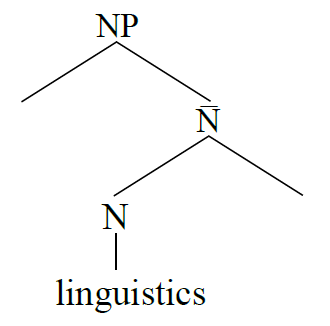
\includegraphics[height=10em]{nouns}
		\begin{forest}
			[NP [.] [N' [N [word]] [.]]]
		\end{forest}
		\caption{Drawing rules (1), (2) and (5) in tree hierarchy}
		\label{fig:nouns-img}
	\end{subfigure}
	\caption{}
\end{figure}
When only one rule is given we still draw two children below each node as in Figure \ref{fig:nouns-img} .

We observe two key properties in PSR and X-Bar theory: First, there is a well-defined structure in the possible syntax trees that we can produce, given by the rules we start with. Second, the rules are capable of recursion -- that is, a rule can reference itself (for example, see rule (2) or (3) in Figure \ref{fig:xbar}). This structure suggests the inklings of a programming language, which also produces highly regulated and recursive forms.
\subsection{Well known homosexual: Alan Turing}
In a foundational paper to the study of computer science as a whole, in 1936 Alan Turing introduced the concept of the \textbf{Turing Machine} (TM), a physical model for computation.\cite{turing1936}  The Turing Machine receives as input an infinite tape of symbols. At any moment the machine reads a single symbol -- referred to as the scanned symbol -- and based on \textit{only} that symbol can then perform several pre-determined options: moving the tape to the left by some number of symbols, to the right, or writing a new symbol in place.

The \textbf{Church-Turing thesis}\cite{kleene1952}
expands upon this, and essentially posits that a Turing Machine is capable of solving any problem that can be computed by an algorithm; and that if there is an algorithm that can solve a problem, then it can be ran by a Turing Machine.\footnote{The concept of a "computable" problem is actually formally defined by what a TM can solve, making my use of the word somewhat circular, but intuitively, it's any problem a human can solve by following instructions and aided by pen \& paper.}

A programming language or rule set is called \textbf{Turing Complete} if it can simulate a Turing Machine, and by the Church-Turing thesis, we know that such languages can determine the solution to any problem that is computable at all -- that is, in terms of which problems they can solve, all Turing-Complete languages are strictly equivalent (even if some are more efficient than others).

The connection between PSR and X-Bar rules to Turing Machines is not a stretch; certain Cellular Automata (CA), such as Conway's Game of Life, are also known to be Turing Complete and exhibit similar properties.\cite{berlekamp2001}
In CA, an initial set of rules determines exactly how each state progresses, likened to the syntax rules given by X-Bar theory. Furthermore, recursive properties also arise CA in that some cell structures of can replicate themselves or "loop" in their configuration, again similar to the often recursive nature of syntax rules in language.

\subsubsection{Brainfuck}
Besides a TM or CA, another popular Turing Complete instruction set is brainfuck (bf). Instead of an infinite tape, the language utilizes an array of (in its original specification) 30,000 byte cells initialized to zero, an input channel to receive initial bytes, an output channel to write bytes to, and a data-pointer which indicates which position in the array is "active".

The bf language uses eight operations to affect these data structures, given by Table \ref{table:bf} . An input program is a series of these operations/instructions, each being executed sequentially unless otherwise noted.
\begin{table}[H]
\begin{tabular}{l|l}
\textbf{Operation} & \textbf{Action Performed}                                                                \\ \hline
\code{>}      & Move the data pointer to the right                                                       \\
\code{<}         & Move the data pointer to the left                                                        \\
\code{+}                  & Increment the data pointer                                                               \\
\code{-}                   & Decrement the data pointer                                                               \\
\code{[}                 & If the active byte is zero, jump to the operation \textit{after} the next {]} character           \\
\code{]}                & If the active byte is not zero, move to the operation \textit{before} the preceding {[} character \\
\code{.}               & Output the active byte to the output channel                                             \\
\code{,}                 & Set the active byte to be equal to the next byte in the input channel
\end{tabular}
\vspace{1em}
\caption{Brainfuck commands}
\label{table:bf}
\end{table}

It is well-known that this programming language is Turing-Complete.\cite{bf_turing_complete}

\subsection{Combining the two ideas}
Given these observations in X-Bar theory and aided by fundamental definitions of computability listed above, the first goal of this paper is to assign a set of instructions to each individual syntax rule of the English language that X-Bar theory gives us. This then creates a mapping between valid syntax trees and the operation of the assigned instructions; a collection of syntax trees, a series of English sentences, then encodes a computer program. We can then reduce this schema to another Turing Complete language, and represent English sentences as computer programs and computer programs as English sentences.

In linguistics, we define syntax as the set of rules that govern how individual words and phrases combine into well-formed sentences. In computer science, we similarly define the syntax of a programming language as the set of rules that govern how symbols and instructions combine into valid statements and expressions. A programming language produced in this manner then would have syntax (in the computer science sense) equivalent to the syntax of the English language.

Lastly, I'll state here and then iterate again later, that under this strategy the words in a sentence do not matter, only the structure of its syntax. So for our purposes the sentence "Victimized undergraduate students sleep occasionally" would be equivalent to "Colorless green ideas sleep furiously" in its program output. While words alter the \textit{semantics} or meaning of a sentence in language, they do not alter the semantics of the program, which is what it does.

\subsection{Process: Syntax to Programming Language}
Largely, the design and programming work of this project can be ordered in three stages:
\begin{enumerate}
	\item \textbf{Assigning instructions to rules}: Assign computing instructions to X-Bar rules in such a way that there is a mapping from syntactically-correct programs to syntactically-correct syntax trees.
	\item \textbf{Combining rules into programs}. Given a desired program as input, use the assignment scheme to combine X-Bar rules into syntax trees whose encoded computation is functionally equivalent to the input program.
	\item \textbf{Assigning words to syntax trees}. Given a series of syntax trees, assign words to the word/head-level components to create complete, grammatical, English sentences.
\end{enumerate}
The work of each stage feeds into the next, with the first being primarily a design problem, and the latter two a challenge of creating and implementing algorithms that solve their respective tasks.

\section{Assigning Instructions to Rules}
X-Bar theory and the various rules it constitutes is a vast study with no universally agreed upon, singlular standards. Methods exist to expand the rules with language features like tense, complementizer phrases, embedded clauses, double objects, and more. \cite{hoekstra1991} \cite{carnie2006}
It is an incredibly powerful theory for modeling syntax generally across language (and not just in English), but any attempt for this model to encompass the entirety of acceptable syntax would be incomplete and overly prescriptivist.

Thus, we begin by limiting ourselves and this project to a choice selection of X-Bar rules, partially listed here in Figure \ref{fig:scope-rules} and completely enumerated in Appendix \ref{app:xbar}.

\begin{figure}
\[
\begin{array}{rllr}
	\textbf{Sentence rules}\quad \psrule{SP}{DP \quad VP}
	\textbf{Determiner rules}\quad \psrule{DP}{DP \quad Conj \quad DP}
\psrule{DP}{Pronoun}
\psrule{DP}{D'}
\psrule{D'}{D \quad NP}
\psrule{D'}{NP}
\psrule{D'}{NP}
\psrule{DTVDP}{DP \quad DP}
	\textbf{Noun rules}\quad \psrule{NP}{N'}
\psrule{NP}{NP \quad Conj \quad NP}
\psrule{N'}{AP \quad N'}
\psrule{N'}{N' \quad PP}
\psrule{N'}{N}
	\textbf{Verb rules}\quad \psrule{VP}{V'}
\psrule{VP}{VP \quad Conj \quad VP}
\psrule{V'}{V' \quad PP}
\psrule{V'}{V' \quad AdvP}
\psrule{V'}{AdvP \quad V'}
\psrule{V'}{TV \quad DP}
\psrule{V'}{DTV \quad DTVDP}
\psrule{V'}{V}
\end{array}
\]
\caption{Partial list of the X-Bar rules in the scope of this project}\label{fig:scope-rules}
\end{figure}
This list was primarily structured around the X-Bar rules in the textbook "Syntax: A Generative Introduction" by Andrew Carnie. \cite{carnie2006}
A few adjustments and simplifications to typical X-Bar rules are made: First, conjugation is ternary, not binary (as first proposed in Chapter 6 of the textbook). This doesn't vastly change the program but does simplify the linguistics of conjugation. Second, and similarly, double objects to ditransitive verbs (labeled "DTV", rule 20) are combined into their own rule ("DTVDP", rule 8) to keep the encoding binary, and again, to simplify the linguistics.

Not included in this list are adjective rules (AP phrases), adverb rules (AdvP phrases), and prepositional rules (PP phrases).

\subsection{Artistic Goals}
I began with the following "artistic goals" that I wanted to achieve in my encoding schema:
\begin{enumerate}
	\item \textbf{Encoding depends on tree structure}. Converting a syntax tree into a flow of instructions should directly utilize the structure of the tree. I do not want a "trivial encoding", where perhaps each word of a specific part of speech corresponds to an individual instruction. Many of the rules in a syntax tree do not contain words, so such an encoding would ignore these rules and their structure entirely. A tree has dimension and its shape should influence the program flow.%\footnote{I mean, I tried I "trivial encoding" first and I couldn't get it to work. But this goal also allows syntactically-ambiguous sentences to have different programs depending on their interpretations.}
		\item \textbf{Variety in resulting sentences}. For a typical program, the generated syntax trees should yield varied sentences that are interesting to read and use all parts of the language. For example, an encoding where adjective rules were rarely utilized would feel disappointing, as would an encoding that required all sentences to have prepositional phrases.
		\item Syntax trees should be "\textbf{efficient}" in how many trees are required to encode a given algorithm. This is a very relative goal -- the number of steps to execute an algorithm in a TM is far greater than the steps needed to execute a functionally equivalent algorithm in assembly code -- but ideally the simplest algorithms one might want to implement do not explode into hundreds of required sentences.
\end{enumerate}
\subsection{Assignment Outline}
I attempted other methods before finally settling on this approach: We proceed by assigning \textbf{bf operations} to each individual X-Bar rule. A syntax tree is converted into a program by (somewhat arbitrarily) \textbf{traversing the tree in-order}, and with each node that we come across, we insert its respective bf operations into our program string (operations that are the same for all nodes with that type of rule). This allows us to convert the "multidimensional" structure of a tree into the one-dimensional structure of a program string, while still preserving the tree topology in this process. Figure \ref{fig:tree-encoding} gives an example.`

\begin{figure}
  \centering
  %\includegraphics[width=0.5\textwidth]{example-image}

	\centering
	\begin{subfigure}[b]{0.45\textwidth}
		\centering
		\begin{forest}
			[SP $\rightarrow$ DP VP [DP $\rightarrow$ Pronoun \code{<<<<}  [Pronoun] [.]] [VP $\rightarrow$ V' \code{>}  [.] [V' $\rightarrow$ V [V] [.]]]]
\end{forest}
		\caption{Syntax tree encoding the bf program \code{<<<<>}, equivalent to \code{<<<}}
	\end{subfigure}
	\hspace{0.02\textwidth}
	\begin{subfigure}[b]{0.45\textwidth}
		\centering
	\begin{forest}
%		[S $\rightarrow$ DP VP [DP $\rightarrow$ D' [.] [D' $\rightarrow$ D NP [D] [NP $\rightarrow$ N' \code{>}  [.] [N' $\rightarrow$ AP N' \code{+}  [AP $\rightarrow$ A' \code{+}  [.] [A' $\rightarrow$ AdvP A' \code{-}  [AdvP $\rightarrow$ Adv' [.] [Adv' $\rightarrow$ Adv \code{-}  [Adv] [.]]] [A' $\rightarrow$ A \code{+}  [A] [.]]]] [N' $\rightarrow$ N \code{<}  [N] [.]]]]]] [VP $\rightarrow$ V' \code{>}  [.] [V' $\rightarrow$ V [V] [.]]]]
		[NP $\rightarrow$ N' \code{>}  [.] [N' $\rightarrow$ AP N' \code{+}  [AP $\rightarrow$ A' \code{+}  [.] [A' $\rightarrow$ AdvP A' \code{-}  [AdvP $\rightarrow$ Adv' [.] [Adv' $\rightarrow$ Adv \code{-}  [Adv] [.]]] [A' $\rightarrow$ A \code{+}  [A] [.]]]] [N' $\rightarrow$ N \code{<}  [N] [.]]]]
	\end{forest}
		\caption{Syntax tree encoding the bf program \code{>+--++<>}, equivalent to \code{>+}.}
	\end{subfigure}
  \caption{Example syntax trees and their programs}
  \label{fig:tree-encoding}
\end{figure}

\subsection{Implementation}
I was unable to find a schema that allowed arbitrary bf programs to be represented by a \textit{single} sentence with my selected X-Bar rules, mainly due to the restrictions imposed by the English syntax. For example, assume we assign any adjective rule the bf operation $X$, and any N' rule the operation $Y$. Because the only rule that introduces adjective phrases is $\textit{N'} \rightarrow \textit{AP} \quad \textit{N'}$, all operations $X$ must be followed by an operation $Y$ in our encoded program. The only operations in bf that satisfy this property is \code{[} and \code{]} -- loops -- but \textit{in between} each loop guard we need to be able to encode every other possible operation. We simply run out of X-Bar rules if we try to make this work. If we picked operations besides \code{[} and \code{]} for $X$ and $Y$, say \code{>} and \code{-}, we'd have that every \code{>} instruction must be followed by a \code{-} which is not necessarily true in bf programs either. We arrive at similar, seemingly unresolvable challenges with other rules.

The notion of \textit{functional equivalence} offers us a way out. For those familiar with bf, we observe that the operations \code{+} and \code{-}, \code{>} and \code{<}, are "reversible" and pairwise inverses of each other. Any bf program composed of these operations can be entirely undone by mirroring/reversing the program and then inverting each operation. For example, the program \code{>>+>-}, which moves the data pointer right twice, increments, moves right once more, decrements, can be undone by its inverse \code{+<-<<}; we immediately increment our previous decrement, move left, undo our first increment, then move to our original position. The two programs \code{+} and \code{>>+>-+<-<<+} are functionally equivalent since their final states are the same, even if the latter one uses more total operations.

While X-Bar rules do create some minimal restrictions for sentences -- for example, every sentence must be composed of a determiner phrase (which includes a noun) and a verb phrase (which includes a verb), we have plenty of \textit{choices} as well. We can choose to use adjectives, to use conjugation, to add on prepositional phrases, which verb form we use, etc. Thus, I assigned the required structural components of a sentence (nouns, verbs, etc) operations like \code{>} and \code{<} (an invertible pair of bf operations I chose more by art than science), and the optional components the un-invertible operations like \code{[} \code{]} \code{.} and \code{,}. Thus we're never forced to use an un-invertible operation, and if we must encounter a \code{>} or \code{<} operation in our X-Bar rules where we do not want one in our final program, we're able to reverse it either elsewhere in the same sentence or in the previous/next sentences.

Finally, by observing typical bf programs, we note \textit{repeated instances} of the same operations. In a corpus I compiled and analyzed, I found that \code{>} appears on average 7 times in a row each time, \code{+} three times in a row, etc. For greater efficiency, I assigned bf operations of greater run lengths to X-Bar rules with a lower recurrence period. For example, \code{+} appears quite often in a program, and adjectives can be stacked one on top of the other (i.e, "the scheming quick brown cunning fox"), so in my final assignment the simplest adjective phrase encodes the instructions \code{+++}. This also makes the resulting sentences very flowery, a property we'll later enjoy the effects of.

A complete list of my X-Bar rules and the operations I assigned them can be found in Appendix \ref{app:xbar}. The average run lengths of bf operations in my corpus can be found in Appendix \ref{app:bf-runs}.

\subsection{Limitations}
This mapping is not bidirectional. While every syntactically-correct ("valid") bf program can be equivalently encoded in syntactically-correct English sentences (see Appendix \ref{app:examples} for a proof), not every syntactically-correct English sentence yields a valid bf program. First, I note again that X-Bar theory or any model of language will always be incomplete, and the notion of "syntactically correct" in linguistics is fuzzy at best, overly prescriptivist at worst. But second, for a bf program to be valid, every \code{[} operation must be paired with one \code{]} operation -- while my schema permits invalid bf programs by allowing these operations to be unmatched.
\section{Combining Rules into Programs}
With a proper schema we're well positioned to start combining rules into programs. I outline the abstract function \code{find\_bf} -- we take a bf program as input, and output a collection of X-Bar syntax trees that encode a functionally equivalent program. We desire two properties from this algorithm: (1), that the resulting syntax trees have \textbf{minimum length}, and (2), that the algorithm completes in a reasonable time, i.e is \textbf{efficient}.

We formalize these notions. The length of a syntax tree could be the number of nodes it contains, but given that when we represent it as a sentence only the word-level nodes are shown to a reader, I'll state that we want to \textit{minimize the total number of words}. Efficiency, I'll define as a \textit{linear runtime} in the length of the input program. Essentially that means that just by repeatedly scanning the input program and then performing a constant number of additional operations, we can come up with an answer.

The goals "smallest encoding" and "fast runtime" are a bit at odds with each other, so we'll likely settle on a heuristic approach for length that still ensures us efficiency.\footnote{The original problem goals are  NP-hard. Proof: it's \textit{probably} correct; exercise for the reader} Consider a perfect algorithm \code{find\_bf'} that is guaranteed to give us minimum length syntax trees for any input, but has non-linear runtime. If we implement \code{find\_bf} by repeatedly calling \code{find\_bf'} on \textit{constant-sized} chunks of our input program, and then just concatenate those outputs together, we get runtime that's linear in the number of chunks, i.e linear in program length. While each collection of syntax trees is optimal for its chunk, the combined syntax trees may not be necessarily optimal for the original input, but it's still probably pretty small.\footnote{In all of my implementations, my "chunking program" is still not optimal but this communicates the rough idea of why the overall runtime is linear, just with \textit{large} constants.}

\subsection{First approach: Graph Search}
We begin by identifying our search space. What are all possible sentences our rules can create? I created a \textit{Recursive Tree} of my X-Bar rules where a \textit{choice-node} connects each set of nodes of the same rule, i.e all $X$ rules. At choice-nodes we may choose which of these rules to use next. A \textit{rule-node} represents the individual rules themselves, which are connected to their respective left and right trees. As rules can be recursive (for example, $\textit{N'} \rightarrow \textit{AP} \quad \textit{N'}$), some nodes are connected either back to their own choice nodes, or elsewhere to a previous position in the tree. Figure \ref{fig:rule-tree} draws part of this tree.

\begin{figure}
  \centering
  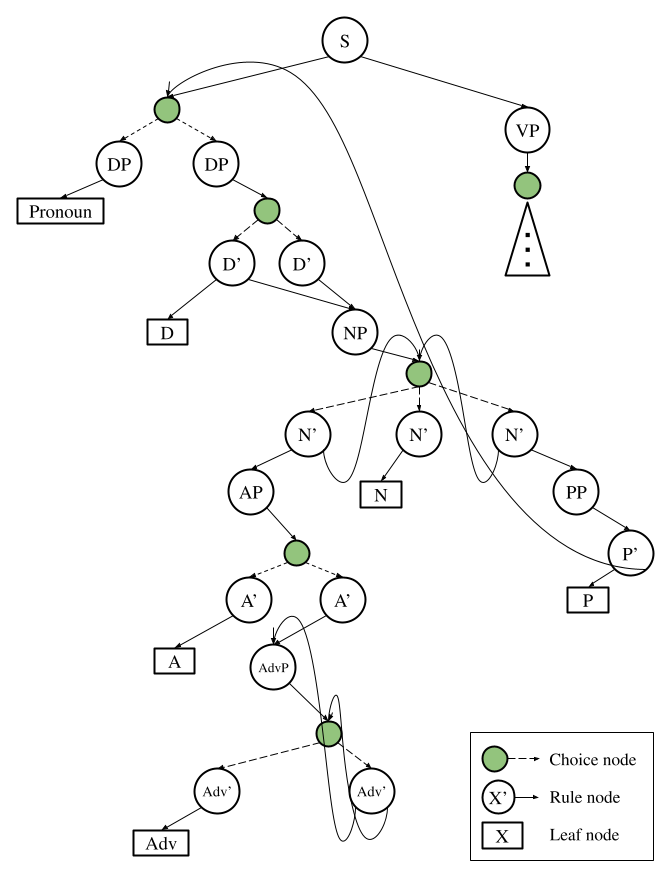
\includegraphics[width=0.5\textwidth]{X-Bar Rule Tree}
	\caption{X-Bar rules laid out in Recursive Tree format (VP subtree and conjugation rules omitted)}
  \label{fig:rule-tree}
\end{figure}

An in-order traversal of the tree is as follows: For any choice node, choose a child to traverse to next. At any rule-node $X \rightarrow Y \quad Z$, we traverse the left subtree rooted at the choice node for $Y$. We add any bf operations we assigned to $X \rightarrow Y \quad Z$ to our program string. Then, we traverse the right subtree of $Z$. We begin traversal at the rule-node $S \rightarrow DP \quad VP$ node. Completing this process and preserving the edges between rule-nodes constructively yields a syntax tree. Any syntax tree/sentence our X-Bar rules permit can be thought of as being produced in this manner.

\subsubsection{Converting the Recursive Tree into a Directed Graph}
Powerful algorithms already exist in computer science for searching graphs. However, "the in-order traversal of a self-recursive binary tree" (this mess we've gotten ourselves into) is itself something entirely different. We want to create a \textit{directed graph} such that the out neighbors of any vertex always represents the next nodes that we could traverse to, in a valid in-order traversal of our recursive tree. Paths in the Directed Graph directly map to in-order traversals of our Recursive Tree, which is again equivalent to building a syntax tree. Whenever we can complete a syntax tree,  we add a neighbor to our original root vertex in the graph to start again with a new sentence.

The program for doing this graph construction is given in its entirety with the code for this project (in the file \code{graph\_search.py}), but some ideas will be outlined here. As computer scientists, we gain intuition in noting that an in-order tree traversal can be implemented by pushing the current node to a stack\footnote{A fundamental data structure in computer science. You can add data to it by "pushing" or remove data by "popping". Items are popped in reverse order of being pushed (last in last out)}, then moving left if we're able to, otherwise popping from our stack and moving right.

A vertex in our Directed Graph represents a state in the Recursive Tree. Each vertex keeps track of its X-Bar rule and a stack of stacks that I call the \textit{commitments} of the vertex, which tracks the heads of rules we've seen and in which "scopes". Each stack in our \code{commitments} is a scope that we enter by pushing onto the outer-stack, and leave by popping. We also have a boolean marker letting us know if the left subtree has already been explored or not.

\begin{tcolorbox}[colframe=black,colback=white,boxrule=0.5pt,arc=2pt]
\textbf{Definitions} \textit{Classes and parts of X-Bar rules}
\begin{enumerate}
	\item A \textbf{leaf} is a part of a rule that is either word-level or has no children. So $D$ is a leaf in the rule $D' \rightarrow D \quad NP$, or the $NP$ rule can be expressed as $NP \rightarrow Leaf \quad N'$, equivalent to $NP \rightarrow N'$.
	\item A rule is an \textbf{exit rule} if its rule has the form $X \rightarrow Leaf \quad Leaf$. Most word-level rules are exit rules.
	\item A rule is an \textbf{left-recursive} if it has the form $X \rightarrow X \quad Y$
	\item The  \textbf{head} of the rule $X \rightarrow Y \quad Z$ is $X$
\end{enumerate}
\end{tcolorbox}

Note that when we encounter an exit rule we jump to some other area in our Recursive Tree traversal. Perhaps the most dramatic jump in Figure~\ref{fig:rule-tree} is that from the rule \mbox{$N' \rightarrow N$} to the $VP$ node (switching from the subject in a sentence to the verb).

For simpler moves, note that if we go the exit rule $A' \rightarrow  A$, we can jump back up the Tree to the rules \mbox{$A' \rightarrow A' \quad Conj \quad A'$}, \mbox{$AP \rightarrow AP \quad Conj \quad AP$}, or \mbox{$N' \rightarrow AP \quad N'$}. If we say "quick", we can choose to either move on to say something like "quick and brown", or go to something like "quick fox". But we can't skip to say, starting a verb phrase from the subject adjective "quick". And if we say "quick fox", we can't then go back and say something like "quick fox and brown", where "and" modifies the adjective. We've lost the ability to make a choice we had access to earlier. Why is this?

Our \textit{commitments} stack again keeps track of which scope we're in. Whenever we come across a rule with a left leaf, we push its head onto the current scope stack --  the last stack in \code{commitments} . Every time we recurse on/traverse a left subtree, we push a \textit{new scope} to \code{commitments}. Whenever we arrive at an exit rule of a left subtree, we can go to any left-recursive rule-node for the head of a rule in our current scope (i.e, "The quick \textit{and brown}", popping within the last stack), staying in that scope. Or, we can "exit" the scope to the previous one ("The quick \textit{fox}", popping off a scope stack entirely from our \textit{commitments}). In the neighbor vertex we next move to, we mark the left subtree of its rule as explored and recurse right. For our syntax tree to terminate we need to exit all scopes we enter -- whenever we recurse left, we're \textit{committed} to eventually return to the rule that we started from. The syntax of a sentence can thus be reduced to a series of choices based on the scopes we're committed to. We build our Graph around this property.

Note that this perhaps models what happens as we're speaking. If we \textit{choose} to say an adjective, then we commit ourselves to following with either more adjectives, and eventually/or, a noun. While traversing the Recursive Tree requires us to make our choices \textit{before} we get to our word-level nodes, our Directed Graph paths allow us to do this \textit{after} we've a word, allowing us greater flexibility in syntax tree construction. This greatly reduces backtracking as we search for trees with the properties that we want, namely, trees whose equivalent programs are similar to the one we're trying to build.

\subsubsection*{A* search}
Once a graph, we can run the A* search algorithm on our graph. A* is a search algorithm typically used to find the shortest path in a graph. We start at some root point and then consider all of its neighbors. We compute the actual cost to get to said neighbor (distance from the previous vertex), as well as a \textit{heuristic} that estimates how close the neighbor is the final goal. At each point in the algorithm, from all possible ways we can expand the vertices we've already explored, we pick whatever neighbor has the lowest expected cost (the actual cost + heuristic cost).

We implement \code{find\_bf'(bf)} as an A* search, where we search for a syntax tree that is functionally equivalent to the input program \code{bf} (without loss of generality we can assume \code{bf} is a simplified bf program).

For A* to work we define the following functions (let \code{v}  be a vertex and let \code{bf}  be the bf program we're trying to encode)
\begin{enumerate}
	\item \code{get\_neighbors(v)}: the neighbors of a vertex
	\item \code{is\_goal\_reached(v, bf)}: whether or not we've reached our goal and can terminate search
	\item \code{distance(v1, v2)}: distance between two vertices
	\item \code{heuristic(v, bf)}: the heuristic cost estimate function from above, how far we think we are from the goal
\end{enumerate}


\code{get\_neighbors(v)} is just the neighbors of a vertex in the Directed Graph that we built earlier.

For \code{is\_goal\_reached(v, bf)}, we return true if the following two conditions are met: (1) Our current syntax tree is complete. We know this is true if we have nothing that we're still committed to in our \code{commitments} stack. And (2), the program our syntax tree encodes is functionally equivalent to \code{bf}.

Since we want to find syntax trees of minimum length, the \code{distance} between two vertices is 1 if the vertex rule we're going to has a word in it, and $\epsilon$ otherwise for some small number $\epsilon$. We have to add that $\epsilon$ so that our search program doesn't just infinitely progress down some chain of nodes with rules that don't affect our encoded program.

And finally, the \code{heuristic(v, bf)} is how we encourage A* to look for syntax trees that are getting closer to our encoded program. Let $bf_v$ be the partial program that the collection of syntax trees for $v$ encodes. We measure $bf_v$ compared to \code{bf} up to the point of their deviance. For any invertible operation that's still left in $bf_v$ after that point, we increase a \code{cost} variable -- this represents a distance that we'll have to travel to "undo" that operation. For any un-invertible operation, we increment \code{cost} by infinity. This means we just made a wrong choice. Then, for any operation that's still left in \code{bf}, we increase \code{cost} as well.

\subsubsection*{Results}
When actually implemented, this approach has several problems that yield limited results. To understand why we first observe some properties about our search mechanism. The A* algorithm  is like filling up a basin with water until the liquid's surface reaches some point on the enclosing walls that we're looking for. The level of the water is the combined heuristic and distance scores. For the water to get to a certain height, it has to get to every accessible level below that one. Or, if the water starts pouring out into some lower basin it finds a way to connect to, it'll fill up the second basin before uniformly rising higher once again.

In our assignment of bf operations to X-Bar rules, we noted that direct paths between each bf operation were often not possible, so we'll regularly need to walk our syntax tree back in the "wrong" direction, then proceed with a path that inverts the intermediary operations thas wellat we're required to pass through before finding the operations we actually want in our final program. We have some low elevation chasm in our basin that we're looking for, but first we need to "flood the search space", or fill the water level high enough so that we can start flowing into that new area. We may be on the path to a smallest syntax tree, but as soon as we run into an operation we need to undo later, our heuristic penalizes us, so the algorithm must try every other path before realizing the previously penalized path was the best option, then correctly proceed with that.

For the bf operations that are more commonly assigned to rules in our syntax tree and more easily undone, this approach works relatively well, just somewhat slow in terms of how fast computers can be. But for the more rare operations (in my assignment, \code{[} and \code{]} especially), we have to search a much wider search space first, to not only find those operations at all, but to also find a path to those operations that also inverts all the intermediary operations required to use \code{[} and \code{]} in our rule assignment. The time it takes to do this is exponential on number of intermediary operations. In these cases this approach was inefficient enough as to become unusable.
\subsubsection*{Memoization?}
One thing I noted is that the A* algorithm will repeatedly find itself in similar positions to ones it's already "solved" before. For example, consider the desired program \code{+++>>+ ++> +++>>+} (spaces just used as a visual separator). The substring \code{+++>>+} is repeated twice. Our algorithm will find a path through our Directed Graph that produces syntax trees that are functionally equivalent to that substring, which may take some time, do some other operations, then do the exact same thing again. We would hope it would be faster on the next pass-through but the algorithm has no concept of learning, and just reconstructs a path from first principles again.

Memoization in computer science might help us here, the concept of saving work for subproblems that an algorithm has already solved once, and then using those subproblems to solve the larger problem entirely.

What are our subproblems? Again, our algorithm translates inputted programs into syntax trees for \textit{sentences} that represent those programs. We can break down a collection of sentence syntax trees, into trees for individual sentences as well as individual phrases or rules. For example, every time our search algorithm builds a complete DP tree, we would save that phrase tree and the part of the program it encodes. The next time we start at a DP node, we can either search through the Recursive Tree again, or just substitute the saved phrase tree we computed earlier.

\begin{tcolorbox}[colframe=black,colback=white,boxrule=0.5pt,arc=2pt]
\textbf{Connection to Linguistics} \textit{Memoization vs constituency and substitution}

Subproblem memoization in this way is actually quite similar to another concept in linguistics: \textbf{constituency} and \textbf{substitution}. Consider our test sentence again, "The quick brown fox jumped over the lazy dog". We can substitute "The quick brown fox" with just "The fox" and still get a syntactically correct sentence. Or, "\textit{It} jumped over the lazy dog", or "\textit{Martha} jumped over the lazy dog", etc. However we couldn't replace just "fox" with "it" and have a correct sentence ("\textit{the it}$^*$ jumped over the lazy dog"). This suggests that all of our substitutions belong to the same class of phrase (in this case, determiner phrases), and we conclude that we can swap phrases out for other phrases of the same class and still preserve syntactical correctness. This is what memoization is doing -- saving the complete phrases that we've already seen before and allowing them to be correctly inserted wherever we can use a  phrase of the same type.
\end{tcolorbox}
Surely this strategy, seemingly justified by both conventional computer science wisdom \textit{and} linguistics, would save our algorithm, right? Unfortunately, after implementing memoization my program became slower overall. Adding more choices to our graph -- choosing to use the subtrees for phrases we've seen before -- increased the \textit{branching factor}, which is generally a negative quality in graphs being searched by A*. Just like humans, algorithms may as well freeze up when given more options to choose from.

\subsection{Second approach: Tree Search}
The Graph Search approach was founded on several powerful ideas, like leveraging an existing search algorithm, creating more flexibility in our program search by delaying choices, and utilizing memoization to reduce repeated computation. However it struggled in a key way: whenever we needed to traverse and undo intermediary operations required to access an operation we desired for our program, we would have to find this path by trying all other paths in the region before we could conclude that temporarily going off track from our goal program was the right move. Furthermore, this process would be extended exponentially based on the number of operations that needed to be inverted. My \textit{Tree Search} approach resolves most of these issues and more.

The basic idea is rather than search for the entire goal program ($bf_{goal}$) all at once, we search for \textit{individual} sentence trees whose programs ($bf_{T}$) contain a high overlap with our goal program. Ideally $bf_T$ is a perfect substring of $bf_{goal}$. We would then split $bf_{T}$ around its overlap with $bf_{goal}$ into a left and right program, then we recursively find syntax trees that solve those smaller programs. Repeating this process builds a Binary Tree where each node is itself a syntax tree. Because each program is constructed via the in-order traversal of its own syntax tree, we construct the final program for $bf_{goal}$ by arranging each sentence-level syntax tree according to an in-order traversal of the "meta" Binary Tree.

It's possible $bf_{T}$ is not a perfect substring however. For example, if $bf_{T}$ has extra operations on the right that aren't in $bf_{goal}$, we call this the \textit{right-remainder} of the program (with a respective left-remainder possibility as well). In this case, when we recurse, in our right subprogram case we prepend the inversion of the right-remainder. When we append the recursive subprogram to the right of $bf_{T}$ this will undo the incorrect remainder portion.

\begin{figure}
  \centering
	\begin{subfigure}[b]{0.45\textwidth}
		\centering
		\begin{forest}
		[$bf_T$: \code{>[-} [\code{>>} ] [\code{]>} [ ] [\code{<} ]]]
	\end{forest}
	\caption{Binary Tree for finding \code{>>>[-]} }
	\end{subfigure}
	\begin{subfigure}[b]{0.45\textwidth}
		\centering
		\begin{enumerate}
			\item Looking for \code{>>>[-]}. Found \code{>[-}
			\begin{enumerate}
			    \item \textsc{Left}. Looking for \code{>>}. Found \code{>>}
					\item \textsc{Right}. Looking for \code{]}. Found \code{]>}
						\begin{enumerate}
						    \item \textsc{Left}. Doing nothing.
						    \item \textsc{Right}. Looking for \code{<} to undo extra \code{>}. Found \code{<}.
						\end{enumerate}
			\end{enumerate}
		\end{enumerate}
		\caption{Program recurrence}
	\end{subfigure}
	\caption{Each node in the Binary Tree represents a syntax tree encoding that program. On line 1.b we have a right-remainder of \code{>}. }
  \label{fig:binary-tree}
\end{figure}

On a macro, sentence-by-sentence level this rewards making necessary "mistakes" (deviations from the goal program) and then fixing them, an improvement from Graph Search. We can also build our program starting at any point, rather than just progressing linearly left to right as Graph Search did, giving us more flexibility. Similar to Graph Search though, the algorithm for finding an optimal tree for $bf_{T}$ is still based on A*, but also improved. We construct a graph to run A* on.

\subsubsection*{Building the graph}
As before the vertices in our graph represent syntax trees, and the neighbors represent ways we can expand that current tree. First, we begin by presenting all possible X-Bar rules as possible starting points to the A* search algorithm. These represent nodes in the syntax tree we'll be constructing, these are the starting "root nodes". The root in a tree is the highest point. For any tree, if either its root or a node below its root is incomplete, we connect the tree's vertex in our graph to all nodes that immediately fill the incomplete space. To prevent too many choices in our graph though we only ever focus on at most one incomplete node at a time.

If the syntax tree is \textit{complete}, i.e the lowest levels of the tree are all leafs/word-level nodes, then we expand the tree upwards; we look at what rules the current root node can be a child of and add those as possible ways to grow the tree. If the tree is complete and the root node is not a possible child of any other rules, we mark the tree as a possible ending point for the program. The only rule that has this property in my X-Bar rules is $S \rightarrow DP \quad VP$, i.e, we can only end if our syntax tree represents a complete sentence.

%TODO: figure
% show like, three images. one of a tree with an incomplete node
% one of the tree once we fill the incomplete node with a word
% one of growing the tree from its root to the top
\begin{figure}
  \centering
	\centering
	\begin{subfigure}[b]{0.30\textwidth}
		\centering
		\begin{forest}
			[N' $\rightarrow$ AP N' [AP $\rightarrow$ A' [\text{Leaf}] [A' $\rightarrow$ A [A] [\text{Leaf}]]] [\textit{None}]]
\end{forest}
		\caption{Starting tree with incomplete node below root}
	\end{subfigure}
	\hspace{0.01\textwidth}
	\begin{subfigure}[b]{0.30\textwidth}
		\centering
		\begin{forest}
			[N' $\rightarrow$ AP N' [AP $\rightarrow$ A' [\text{Leaf}] [A' $\rightarrow$ A [A] [\text{Leaf}]]] [N' $\rightarrow$ N [N] [\text{Leaf}]]]
\end{forest}
\caption{Fill incomplete node with \mbox{$N' \rightarrow N$}, yielding complete tree}
	\end{subfigure}
	\hspace{0.01\textwidth}
	\begin{subfigure}[b]{0.30\textwidth}
		\centering
		\begin{forest}
			[N' $\rightarrow$ AP N' [\textit{None}] [N' $\rightarrow$ AP N' [AP $\rightarrow$ A' [\text{Leaf}] [A' $\rightarrow$ A [A] [\text{Leaf}]]] [N' $\rightarrow$ N [N] [\text{Leaf}]]]]
\end{forest}
\caption{Grow tree upwards with \mbox{$N' \rightarrow AP\ N'$}}
	\end{subfigure}
  \caption{Example of a possible path in our Tree Search graph}
  \label{fig:tree-search-graph}
\end{figure}

\subsubsection*{A* Search Heuristic}
Again, the goal of A* in Tree Search is to find the syntax tree for an individual sentence whose program operations have the greatest overlap with our goal program. Rather than count overlap based on the number of common operations, however, we assign each operation a weight roughly based on how many intermediary operations we need to pass through (and later undo) to access it. We find the common overlap between $bf_{T}$ and $bf_{goal}$ where the sum of weights of each character in the overlap is maximized (greatest cost substring).\footnote{Because A* looks for \textit{shortest} or \textit{cheapest} paths, we multiply this total value by -1. Smaller is better.}%  If we're looking for an operation like \code{[}, which is often buried in the surrounding sentence, we assign it a favorable weight

Usually in A* the \code{heuristic} function -- which estimates a distance to the goal -- is strictly positive. Recall the analogy about filling a basin with water, where the water fills up all accessible regions of lower elevation before rising upwards. If we assign negative weight to the things that we want in our $bf_{T}$ program, we can essentially get the water to flow downhill, which is faster. And if we assign a negative weight of greater magnitude for an operation that involves more intermediaries we have to invert, then we can coax our water into a local minimum pool, which fills up with water as we find a way to undo the unwanted operations.

Furthermore, we don't just care about overlap between $bf_{T}$ and $bf_{goal}$; we also want to minimize the operations in $bf_{T}$ that aren't in $bf_{goal}$ (the left and right remainder, from earlier). We use a separate, less-harsh weighting scheme for these "mistakes". Namely, in most instances we don't penalize \code{>} and \code{<} since by design, we assigned these to the structural components of the sentence that we can't help but run into. We expect that we'll undo those operations later. Similar to Graph Search we also assign a weight of $\infty$ to uninvertible operations we don't want in our program string.

Finally, to help prevent finding local minima when better solutions exist, we add a small, unfavorable weight to every finished sentence syntax tree. Using our metaphor, this causes the waters of our A* search to rise again up to a fixed height, just to see if there are any lower elevation regions it can drain into.

The complete code for this and the rest of the project can be found in the file \code{tree\_search.py}.

\subsubsection*{Results}
The code works spectacularly, entirely as desired and orders of magnitudes faster than Graph Search. We trade off some levels of perfection for speed, however; our A* search isn't guaranteed to give us syntax trees of minimum size, but trees are small enough for our needs. For small programs commonly used to undo mistakes (i.e \code{>}, \code{<<<}, etc), I memoize the sentences that correspond to these programs for increased efficiency.

Because of side-effects due to hashing, the algorithm isn't deterministic, so even in between repeated calls to the same goal program, sentences are varied, and for each memoized program I save several possible sentences that are functionally equivalent for more variety.

% TODO: Figure, show a few syntax trees and their corresponding program. Maybe just do leaves, and not show the entire trees?
%\begin{figure}
%  \centering
%  \includegraphics[width=0.5\textwidth]{example-image}
%  \caption{Example of a possible path in our Tree Search graph}
%  \label{fig:tree-search-example}
%\end{figure}
%More example programs and their encoded equivalences can be found in Appendix \ref{app:examples}
Example programs and their encoded equivalences can be found in Appendix \ref{app:examples}

\section{Assigning Words to Syntax Trees}
Now begins the Mad Libs game of filling in each word in the syntax tree.

I started by just picking word banks for each each part of speech: determiners, pronouns, nouns, verbs, adjectives, and adverbs. Naively, for each word in the sentence we can just randomly slot in a word from the word bank corresponding to its part of speech. However this yields a few problems with English grammar. I identified the following rules I wanted to respect:
\begin{enumerate}
	\item \textbf{Pronoun agreement}. Pronouns have three forms: nominative, accusative, and anaphoric. For example, for "I", the respective forms are "I", "me", "myself. For "you", it's just "you", "you", "yourself". I need to find out what the subject of the sentence is, and it's the same as the pronoun in an object, I use the anaphoric form ("I see \textit{myself}"). If it's different, I use the accusative form ("You see \textit{me}"). For the subject, I use the nominative form.
	\item \textbf{Verb conjugation}. Once I know the subject, my verb needs to agree with it. So "You are my friend" is ok, but "You \textit{is}* my friend" is not.
	\item \textbf{Noun pluralization}. Some nouns need to be pluralized based on my X-Bar rules. Some nouns in my wordbank are already plural (like "eyes"), and some nouns are known as \textit{mass nouns}, which do not get pluralized. For example, consider the words "\textit{$<$noun (plural)$>$ $<$verb$>$ $<$determiner$>$ $<$noun$>$}".  We can write "Eyes cover the face", or  "Enthusiasm earns my respect". There's no such thing as "Enthusiasms*", and in the two sentences the verbs "cover" and "earns" are conjugated differently ("Eyes covers* the face" does not work).
\end{enumerate}
To implement these rules I use a system of tags and constraints. Certain X-Bar rules have their own "tags", and all other rules under them in a syntax tree, including words, may inherit them. Individual words can also have their own tags, and may propagate their tags upwards through the tree. Word choice may be modified based on the tags in the current scope.

For example -- when we choose the subject, we create a tag for which person we're in (first, second, or third), then send that tag to all ancestors in our syntax tree. We fill in words left to right, in-order again. When we go to select a verb, the subject tag is already in scope, as well as a possible pluralization tag, which modify the verb we choose accordingly.

There are a few more aesthetic rules I implemented -- alternating the possession in a sentence between "your"/"my" and the person "you"/"I"; making sure certain words aren't repeated where they shouldn't be (ex, we can't use the same adjective twice to describe the same noun); using more refined word-banks in certain situations -- but these are also done through the system of tags, constraints, and modifications.
\section{Love Languages}
In my schema the program that a sentence encodes comes entirely from its syntax tree, with no regard to the individual words. So what kind of words do we want to choose in our sentences? What do we want to say, to not say? We return to another program with similar goals, the 1952 Strachey love letter algorithm, regarded by many as the first work in computer-generated literature. \cite{gaboury2013}

%YOU ARE MY [adjective] [noun]. MY [adjective] [noun] [adverb] [verbs] YOUR [adjective] [noun].
\subsection{Lesser known homosexual: Christopher Strachey}
Christopher Strachey was an early programmer and personal colleague of Alan Turing. They both attended King's College in Cambridge, with Turing beginning his master's the year Strachey started his bachelor's. Despite shared interests in computing the two first met socially.

While Turing conceptualized the field of computer science we know today, Strachey himself was a source of many firsts: first video game (draughts\footnote{"draughts [sic]". \textit{Checkers} is the American-English name of the game}), England's first computer music (the British National Anthem), and the first computer-generated literature.

Strachey's love letter algorithm was programmed on Manchester's Ferranti Mark I computer -- the manual of which was written by Turing. Soon, the university's notice board slowly began populating with printouts, signed "M.U.C" for Manchester University Computer.

\begin{figure}
	\centering
    \begin{verbatim}

DEAR LOVE

 MY CHARM CURIOUSLY HOPES FOR YOUR LIKING. MY COVETOUS AFFECTION IMPATIENTLY
LUSTS AFTER YOUR EAGER ARDOUR. YOU ARE MY LITTLE ARDOUR. MY WISTFUL LIKING LOVES
YOUR DESIRE. MY WISTFUL INFATUATION LONGS FOR YOUR FOND INFATUATION.

                                        YOURS SEDUCTIVELY

                                        M.U.C\end{verbatim}
		\caption{Output from the love letter algorithm using Nick Montfort's reimplementation}\label{fig:muc}
\end{figure}
The letters are overwrought, still dripping from being dunked in and pulled out of a thesaurus. With a reimplementation \cite{montfort2014} of Strachey's algorithm on my computer I can endlessly refresh its results, never once having to worry about exhausting the combinatorial explosion of possibilities but never once really seeing anything new. Undercurrents of longing and desperation guide an experience of reading separate pages ripped from the same book. From Strachey, a queer man with a similar "love life" to Turing, according to the latter's biographer, \cite{hodges1992}
the work has been viewed as a queer critique of heteronormative expressions of affection.

Phrase structure rules weren't conceptualized until 1957, five years after Strachey's algorithm, but even before it didn't take Chomsky's linguistic theory to represent and understand syntax trees. The program plays the same Mad Libs game, with the fixed syntactic structures "YOU ARE MY [Adjective] [Noun]", and "MY [Adjective] [Noun] [Adverbs] [Verbs] YOUR [Adjective] [Noun]". The words are all the same, mostly pulled straight from Roget's thesaurus. It's the syntax that defines the letter.

Given this it's easy to follow along myself. With only a few additions I largely deferred to Strachey's word banks. On on random output, here's how my algorithm represents the bf program for printing "Hello World", just the sentences without their syntax trees:
\footnote{bf itself is an inefficient language, and it's easier to pack single characters onto a screen rather than words. The complete program (166 more words) is in Appendix \ref{app:examples}}

\begin{verbatim}
    I PANT FOR DEVOTION. YOU ARE MY DEAR ARDENT LOVEABLE JEWEL. MY
EAGERNESS AVIDLY AND LOVINGLY AND IMPATIENTLY WINNINGLY SWOONS. I YEARN FOR YOUR
BODY. MY DEVOTION MELTS. MY LOVINGLY FERVENT FONDNESS DREAMS. MY TOTALLY AMOROUS
RAPTURE FLIRTS. YOUR FANCY OFFERS MY AFFECTION YOUR FERVOUR. YOU ARE MY ADORABLE
JEWEL. MY BODY HUNGERS IN LUST AND PINES. YOU ARE MY PRECIOUS COVETOUS HONEY.
YOUR TOTALLY IMPATIENT LIKING DANCES. MY ENCHANTMENT OFFERS YOUR LIKING MY
LONGING. I AM YOUR COVETOUS AFFECTIONATE JEWEL.
\end{verbatim}
%YOUR  TOTALLY AMOROUS TENDERNESS PINES. MY LONGING LEAPS. YOU ARE MY CRAVING DUCK. I SIGH WISTFULLY. MY TENDERNESS AND DEVOTION GAZES. MY ADORATION CLINGS TO YOU. LITTLE EYES TENDERLY FLIRT. PLEASE!. YOUR LOVINGLY EAGER APPETITE FLIRTS. PLEASE!. I THIRST FOR LONGING. YOU ARE MY CRAVING CURIOUS MOPPET. MY INTENSELY TENDER HUNGER GAZES. OH!. OH!. MY FONDNESS GAZES. YOU ARE MY AFFECTIONATE JEWEL. TENDERNESS PROMISES YOU MY ENCHANTMENT. LORD ABOVE!. I CARESS. MY ADORABLE LUST BEAUTIFULLY PINES. LORD ABOVE!. YOUR LUST PRIZES MY INFATUATION. YOU ARE MY FOND LOVING DEAR AMOROUS PASSIONATE DUCK. AMBITION OFFERS YOU MY BODY. LORD ABOVE!. MY ARDOUR CARESSES. PLEASE!. YOUR SYMPATHY FLUTTERS. YOU ARE MY BURNING HONEY. MY LONGING GAZES. OH!. I CARE FOR HUNGER. I AM YOUR TOTALLY PRECIOUS LITTLE DEAR. YOUR ANXIOUS BEAUTIFULLY PASSIONATE THIRST CARESSES. OH!. I SIGH FOR YOUR ENTHUSIASM. MY ADORATION DANCES. MY PRECIOUS WISTFUL FERVENTLY DEVOTED DARLING ENCHANTMENT SWOONS. OH!. I PINE. YOUR VERY DEAR ENTHUSIASM MELTS. OH!. I WANT YOUR THIRST. MY AMBITION YEARNS. OH!
\subsection{Why love letters?}
I conceived of this project in Fall of 2022, its first externalized proof of concept occurring, somewhat embarrassingly, during pillow talk with my then boyfriend. %TODO: do i want this?
Perhaps appropriate origins. Later that year I discovered Christopher Strachey and thought immediately of the tucked-away idea of my programming language. \textit{If the words aren't important to the program, what do I fill them with?} An upcoming student-led presentation showcase, scheduled to be held on Valentine's Day, spurred my first hurried attempt at implementing this. In motivated bursts during the week before, I drew syntax trees in the margins of the math notes, but ultimately couldn't come up with anything.

I committed myself to trying again only years later, beginning the Spring and final semester of my senior year, the 2025 semester of writing this, once again with syntax trees scratched into the margins of my notebooks. I couldn't leave it unresolved. As I navigated the bugs and conceptual challenges, I reasoned more about the project.

If Strachey's algorithm criticizes heteronormative displays of affection as algorithmic, then this process literally turns them into algorithms. If the sentences Love Language generates are reduced functionally to only their syntax, the loving words, despite or maybe even because of their ornateness, contribute nothing to the final result. In computer science the \textit{semantics} of a program is again what it does. In language the semantics of a sentence is its meaning. The latter lens yields only the singular interpretation of a yearning, pining, clinging, longing -- while via the programming semantics, we can communicate anything. The love letter is less a genre of content than of means.

From a different angle, we might personify the process of generation itself, which at this point in the paper we're now familiar with. The A* algorithm, which hurriedly scans through all the things it might say, all the possible variations of expression it can formulate, is a process of rumination. It is the anxious mind of the obsessed lover. And if the failed Graph Search approach is a closer model for human language, we see that often in a desire for perfection, the speaker may say nothing at all. Tree Search, more tolerant of its own mistakes and free from our natural constraint of conveying language linearly, delivers results through methods of its inhumanity.
% connection to modern generative text / AI?

\section{Conclusion}
\begin{wrapfigure}{r}{0.45\textwidth}
\vspace{-4em}
  \begin{center}
    \includegraphics[width=0.43\textwidth]{letter}
  \end{center}
\vspace{-1em}
  \caption{Printed letter in CMU's school of computer science}
\vspace{-2em}
\end{wrapfigure}
Strachey’s algorithm is perhaps a computational proof to the strength of our empathy. One which would invariably fail the Turing test, but maybe still momentarily shock us with its misplaced passion. When I read the outputted letters, unceremoniously printed and easily disposed of on my computer screen, I can’t help but feel a bit bad for the program. The relatively simple code is enough to briefly hold a mirror to our own mental processes. As soon as it starts to communicate on a level of linguistic semantics, Strachey’s algorithm and Love Language become these crude drawings of faces on paper -- but even then I want to speak to them.

I see printing a love letter — and displaying it in a public forum as Strachey did — less as putting some obsessive algorithm in the stocks and more as an honorific. It is the ephemera of a relationship. The repeated observation of the promises and commitments of the sentence. We acknowledge the shortcomings of the machine but still recognize what it reflects in us, the ways it even briefly pulled at our hearts.

Modern computer-generated text is today primarily produced by generative AI. Actual “love programs”, which more naturally conceal the depths of their yearning and the mechanics of their thought, can be readily designed by simple prompting on top of an existing large language model. But in their imprecise proximity to something entirely convincing, I find them less relatable. It’s the same uncanny valley of a wax figure, the black box thought of an alien mind. Strachey’s is honest to a fault, but maybe there’s something to respect in that. Love Language follows suit.

% Bibliography
\bibliographystyle{splncs04}
\bibliography{references} % If you have a .bib file

\newpage
\appendix
\section{X-Bar Rules Used} \label{app:xbar}
The rules $SP \rightarrow EXC$ and $SP \rightarrow QUERY$ are my own and represent "exclamation" and "query" respectively, designed to simplify the rule assignment.
\vspace{1em}

\begin{table}
\setcounter{rulecounter}{1}
\[
\begin{array}{rllrl}
    \textbf{Sentence rules} \quad \psruleop{SP}{DP \quad VP}{}
    \psruleop{SP}{EXC}{.}
    \psruleop{SP}{QUERY}{,}

    \textbf{Determiner rules} \quad \psruleop{DP}{DP \quad Conj \quad DP}{>>}
    \psruleop{DP}{Pronoun}{<<<<}
    \psruleop{DP}{D'}{}
    \psruleop{D'}{D \quad NP}{}
    \psruleop{D'}{NP}{>>>}
    \psruleop{DTVDP}{DP \quad DP}{}

    \textbf{Noun rules} \quad \psruleop{NP}{N'}{>}
    \psruleop{NP}{NP \quad Conj \quad NP}{]}
    \psruleop{N'}{AP \quad N'}{+}
    \psruleop{N'}{N' \quad PP}{}
    \psruleop{N'}{N}{<}

    \textbf{Verb rules} \quad \psruleop{VP}{V'}{>}
    \psruleop{VP}{VP \quad Conj \quad VP}{<<<<}
    \psruleop{V'}{V' \quad PP}{}
    \psruleop{V'}{V' \quad AdvP}{}
    \psruleop{V'}{AdvP \quad V'}{}
    \psruleop{V'}{TV \quad DP}{>}
    \psruleop{V'}{DTV \quad DTVDP}{>}
    \psruleop{V'}{V}{}

    \textbf{Adverb rules} \quad \psruleop{AdvP}{Adv'}{}
    \psruleop{AdvP}{AdvP \quad Conj \quad AdvP}{}
    \psruleop{Adv'}{Adv' \quad Conj \quad Adv'}{++}
    \psruleop{Adv'}{AdvP \quad Adv'}{[}
    \psruleop{Adv'}{Adv}{-}

    \textbf{Adjective rules} \quad \psruleop{AP}{A'}{+}
    \psruleop{AP}{AP \quad Conj \quad AP}{------}
    \psruleop{A'}{A' \quad Conj \quad A'}{--}
    \psruleop{A'}{AdvP \quad A'}{-}
    \psruleop{A'}{A}{+}

    \textbf{Preposition rules} \quad \psruleop{PP}{P'}{>>}
    \psruleop{PP}{PP \quad Conj \quad PP}{>>>>}
    \psruleop{P'}{P \quad DP}{}
\end{array}
\]

\caption{X-Bar Rules used, and their assigned operations}
\end{table}
\newpage
\section{Frequency of Brainfuck Operation} \label{app:bf-runs}
I compiled my corpus somewhat arbitrarily with common bf programs (word count, fibonacci sequence, hello world, an approximation for pi) .

In the following table, "frequency" is how common the operation is in the corpus. Average run length is how many times it's likely to be repeated, when it does show up.

\begin{table}[H]
\centering
\begin{tabular}{@{}l l l@{}}
\toprule
\textbf{Operation}\;\; & \textbf{Frequency (\%)}\;\; & \textbf{Avg Run Length} \\ \midrule
\code{>}  & 20.2  & 6.8  \\
\code{<}  & 17.9  & 7.1  \\
\code{+}  & 30.8  & 3.4  \\
\code{-}  & 11.4  & 1.4  \\
\code{[}  & 7.6  & 1.1  \\
\code{]}  & 7.6   & 1.0  \\
\code{.}  & 4.3   & 1.0  \\
\code{,}  & 0.2   & 1.0   \\ \bottomrule
\end{tabular}
\vspace{1em}
\caption{frequency of each bf operation and average run length}
\end{table}

\newpage
\section{Example Love Letters and Completeness of \textit{Love Languages}} \label{app:examples}
For brevity, complete syntax trees are instead written linearly as just their words. Parentheses wrap all words that are in a common phrase.\\

\noindent
\textbf{bf program:} \code{.+[.+]}\\
writes all printable characters to the console.
\begin{verbatim}
PLEASE!. I YEARN WITH YOUR FANCY. MY TOTALLY DARLING BEAUTIFULLY INCREDIBLY
LITTLE FELLOW FEELING GAZES. LORD ABOVE!. I TEMPT YOUR THIRST. MY EYES SWOON.
YOUR BEAUTIFULLY FOND ENTHUSIASM SIGHS. YOUR FERVOUR AND FONDNESS DREAMS. I
HUNGER ON YOUR HEART.

syntax: EXC ((Pronoun (TV (D N))) ((D N) V)) ((D ((Adv A) (((Adv Adv) A) N))) V)
EXC ((Pronoun (TV (D N))) ((D N) V)) ((D ((Adv A) N)) V) ((D (N Conj N)) V)
(Pronoun (V (P (D N))))
\end{verbatim}

\vspace{1em}
\noindent
\textbf{bf program:} \code{++++++++++[>+>+++>+++++++>++++++++++<<<<-]>>>++.>+.+++++++..+++.<<++.>+++++++++}
\code{++++++.>.+++.------.--------.<<+.<.}\\
prints "Hello World" to the console.
\begin{verbatim}
    I PANT FOR DEVOTION. YOU ARE MY DEAR ARDENT LOVEABLE JEWEL. MY
EAGERNESS AVIDLY AND LOVINGLY AND IMPATIENTLY WINNINGLY SWOONS. I YEARN FOR YOUR
BODY. MY DEVOTION MELTS. MY LOVINGLY FERVENT FONDNESS DREAMS. MY TOTALLY AMOROUS
RAPTURE FLIRTS. YOUR FANCY OFFERS MY AFFECTION YOUR FERVOUR. YOU ARE MY ADORABLE
JEWEL. MY BODY HUNGERS IN LUST AND PINES. YOU ARE MY PRECIOUS COVETOUS HONEY.
YOUR TOTALLY IMPATIENT LIKING DANCES. MY ENCHANTMENT OFFERS YOUR LIKING MY
LONGING. I AM YOUR COVETOUS AFFECTIONATE JEWEL. YOUR  TOTALLY AMOROUS TENDERNESS
PINES. MY LONGING LEAPS. YOU ARE MY CRAVING DUCK. I SIGH WISTFULLY. MY
TENDERNESS AND DEVOTION GAZES. MY ADORATION CLINGS TO YOU. LITTLE EYES TENDERLY
FLIRT. PLEASE!. YOUR LOVINGLY EAGER APPETITE FLIRTS. PLEASE!. I THIRST FOR
LONGING. YOU ARE MY CRAVING CURIOUS MOPPET. MY INTENSELY TENDER HUNGER GAZES.
OH!. OH!. MY FONDNESS GAZES. YOU ARE MY AFFECTIONATE JEWEL. TENDERNESS PROMISES
YOU MY ENCHANTMENT. LORD ABOVE!. I CARESS. MY ADORABLE LUST BEAUTIFULLY PINES.
LORD ABOVE!. YOUR LUST PRIZES MY INFATUATION. YOU ARE MY FOND LOVING DEAR
AMOROUS PASSIONATE DUCK. AMBITION OFFERS YOU MY BODY. LORD ABOVE!. MY ARDOUR
CARESSES. PLEASE!. YOUR SYMPATHY FLUTTERS. YOU ARE MY BURNING HONEY. MY LONGING
GAZES. OH!. I CARE FOR HUNGER. I AM YOUR TOTALLY PRECIOUS LITTLE DEAR. YOUR
ANXIOUS BEAUTIFULLY PASSIONATE THIRST CARESSES. OH!. I SIGH FOR YOUR ENTHUSIASM.
MY ADORATION DANCES. MY PRECIOUS WISTFUL FERVENTLY DEVOTED DARLING ENCHANTMENT
SWOONS. OH!. I PINE. YOUR VERY DEAR ENTHUSIASM MELTS. OH!. I WANT YOUR THIRST.
MY AMBITION YEARNS. OH!\end{verbatim}

We note that Love Language is complete -- i.e can represent any bf program -- if it can construct each operation individually. Then we could simply just represent any program by converting operations individually to these encodings, even if less efficient.

\begin{verbatim}
>
(Pronoun (TV N))
I WISH FOR DEVOTION

<
((Pronoun (TV (D N))) ((D N) V))
I THIRST FOR YOUR DEVOTION. YOUR LOVE CARESSES

+
(Pronoun (V (P (D N)))) ((D ((Adv A) N)) V)
I CARESS BEYOND YOUR FANCY. MY BEAUTIFULLY LOVESICK FERVOUR SWOONS

-
(Pronoun (V (P (D N)))) ((D N) (V Adv))
I GAZE WITH YOUR HUNGER. YOUR HUNGER GAZES TENDERLY

[
((Pronoun (TV (D N))) ((D N) V)) ((D (((Adv Adv) A) N)) V)
I CARE FOR YOUR FANCY. MY LONGING HUNGERS. YOUR TOTALLY INTENSELY CRAVING EYES CARESS

]
((D (N Conj N)) V) ((Pronoun (TV (D N))) ((D N) V))
YOUR FERVOUR AND EAGERNESS SIGHS. I ADORE YOUR LONGING. YOUR LOVE GAZES

.
EXC
PLEASE!

,
QUERY
DO I DREAM?
\end{verbatim}

Download the code for this project and run the executable \code{python main.py} to generate your own sentences: \href{https://cassidydiamond.me/love-languages}{https://cassidydiamond.me/love-languages}
\end{document}

